\section{Turret Test}
The turret was tested using a circular target moving at $0,19$ $m/s$ in a straight line. 
The target was moved away from the turret in 10-cm increments until the turret was unable to hit the target. Starting at 60 cm, 10 test shots were performed at each distance in both left-to-right and right-to-left direction, from the perspective of the turret. A hit or miss was noted, with no regard as to where on the target the projectile hit. The hit ratio is shown below, as a function of distance:

\begin{figure}
	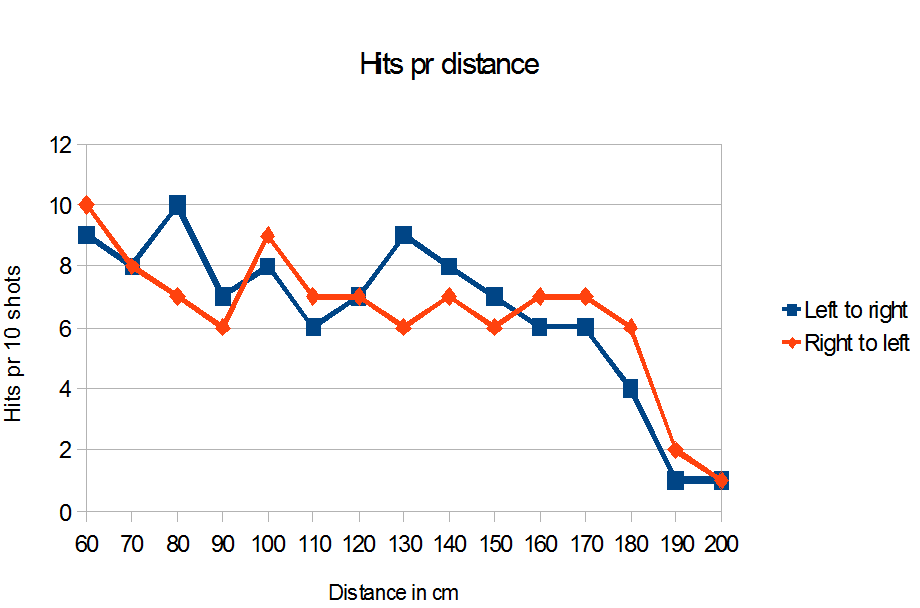
\includegraphics[scale=0.5]{img/test.png}
	\caption{Systematic test data}
	\label{systest}
\end{figure}

As can be seen above, the turret consistently hits the target more than half the time on the 60 - 180 cm range, with the highest hit to miss ratio at the beginning. After 180 cm, which was the predicted maximum range, the turret hits the target only a few times. The accuracy of the turret fluctuates, but it is seemingly more precise early on, which makes sense given that inaccuracies in placement of Kinect relative to turret will become greater the further away the target is moved. Overall the left to right moving target is hit more consistently than the right to left moving target (66\% relative to 64\%), however the right to left moving target is more precise in the 160 cm to 180 cm range. This, we believe, is due to the difference in surface on the two side of the target, with the side facing the turret in the right to left direction being easier to identify precisely at that distance.

The overall hit percent in both directions is 65\%.
